\section{Results and Analysis}

In this section, we present the experimental results and analyze the performance of \model in comparison to the baseline models.

\definecolor{FBest}{RGB}{4,130,53}

\begin{table*}[htbp]
\renewcommand{\arraystretch}{0.9}
\footnotesize
\caption{Performance comparison across all methods using four evaluation metrics. Results highlighted in \textbf{\textcolor{FBest}{green}} represent the best-performing statistic for each model. The improvement row illustrates \model's performance gains over the top-performing baselines.}

\setlength{\abovecaptionskip}{0.1cm}
\centering
\begin{threeparttable}
\setlength{\tabcolsep}{2.5pt}
\resizebox{\linewidth}{!}{ 
\begin{tabular}{clcccclcccclcccc}
\toprule
\multirow{3}{*}{Categories} & \multirow{3}{*}{Models} & \multicolumn{4}{c}{AAPL} & & \multicolumn{4}{c}{GOOGL} & & \multicolumn{4}{c}{AMZN} \\ 
\cmidrule{3-6}\cmidrule{8-11}\cmidrule{13-16}
&& CR\%$\uparrow$ & ARR\%$\uparrow$ & SR$\uparrow$ & MDD\%$\downarrow$ & & CR\%$\uparrow$ & ARR\%$\uparrow$ & SR$\uparrow$ & MDD\%$\downarrow$ & & CR\%$\uparrow$ & ARR\%$\uparrow$ & SR$\uparrow$ & MDD\%$\downarrow$ \\ 
\midrule
Market 
& B\&H& -5.23& -5.09 & -1.29 & 11.90 && 7.78 & 8.09 & 1.35 & 13.04  && 17.1 & 17.6 & 3.53 & 3.80\\
\midrule
\multirow{3}{*}{\begin{tabular}[c]{@{}c@{}}Rule-based\end{tabular}}
& MACD& -1.49 & -1.48 & -0.81 & 4.53 && 6.20 & 6.26 & 2.31 & \textbf{\textcolor{FBest}{1.22}}  && - & - & - & -\\
& KDJ\&RSI& 2.05 & 2.07 & 1.64 & 1.09 && 0.4 & 0.4 & 0.02 & 1.58  && -0.77 & -0.76 &-2.25 & 1.08\\
& ZMR& 0.57 & 0.57 & 0.17 & \textbf{\textcolor{FBest}{0.86}} && -0.58 & 0.58 & 2.12 & 2.34  && -0.77 & -0.77 & -2.45 & \textbf{\textcolor{FBest}{0.82}}\\
& SMA & -3.2 & -2.97 & -1.72 & 3.67 && 6.23 & 6.43 & 2.12 & 2.34 && 11.01 & 11.6 & 2.22 & 3.97\\
\midrule
\multirow{1}{*}{\begin{tabular}[c]{@{}c@{}} Ours\end{tabular}}
& \textbf{\texttt{\model}}& \textbf{\textcolor{FBest}{26.62}} & \textbf{\textcolor{FBest}{30.5}} & \textbf{\textcolor{FBest}{8.21}} & 0.91 && \textbf{\textcolor{FBest}{24.36}} & \textbf{\textcolor{FBest}{27.58}} & \textbf{\textcolor{FBest}{6.39}} & 1.69  && \textbf{\textcolor{FBest}{23.21}} & \textbf{\textcolor{FBest}{24.90}} & \textbf{\textcolor{FBest}{5.60}} & 2.11\\
\midrule
\multicolumn{2}{c}{Improvement(\%)} 
& 24.57 & 28.43 & 6.57 & - && 16.58  & 19.49 & 4.26 & - && 6.10 & 7.30 & 2.07 & -\\
\bottomrule
\end{tabular}
}
\end{threeparttable}
\label{tab:performance}
\end{table*}


\subsection{Performance Comparison}
\subsubsection{Cumulative and Annual Returns}
Table \ref{tab:performance} and Figures \ref{fig:aapl-transactions}, \ref{fig:aapl-cumulative-returns}, \ref{fig:amzn-performance-details}, \ref{fig:amzn-performance-comparison}, \ref{fig:googl-performance-details}, and \ref{fig:googl-performance-comparison} demonstrate that our method outperforms existing rule-based trading baselines, particularly in profitability, as measured by returns. \model achieves at least a 23.21\% cumulative return and a 24.90\% annual return on the three sampled stocks, surpassing the best-performing baselines by a margin of 6.1\%. Notably, on \$AAPL stock—a particularly challenging case due to market volatility during the testing period—traditional methods struggled, as their patterns failed to generalize to this situation. In contrast, \model excelled under these adverse conditions, achieving returns exceeding 26\% within months.



% ICML version
\begin{figure}[htbp]
% \vskip 0.2in
\begin{center}
\centerline{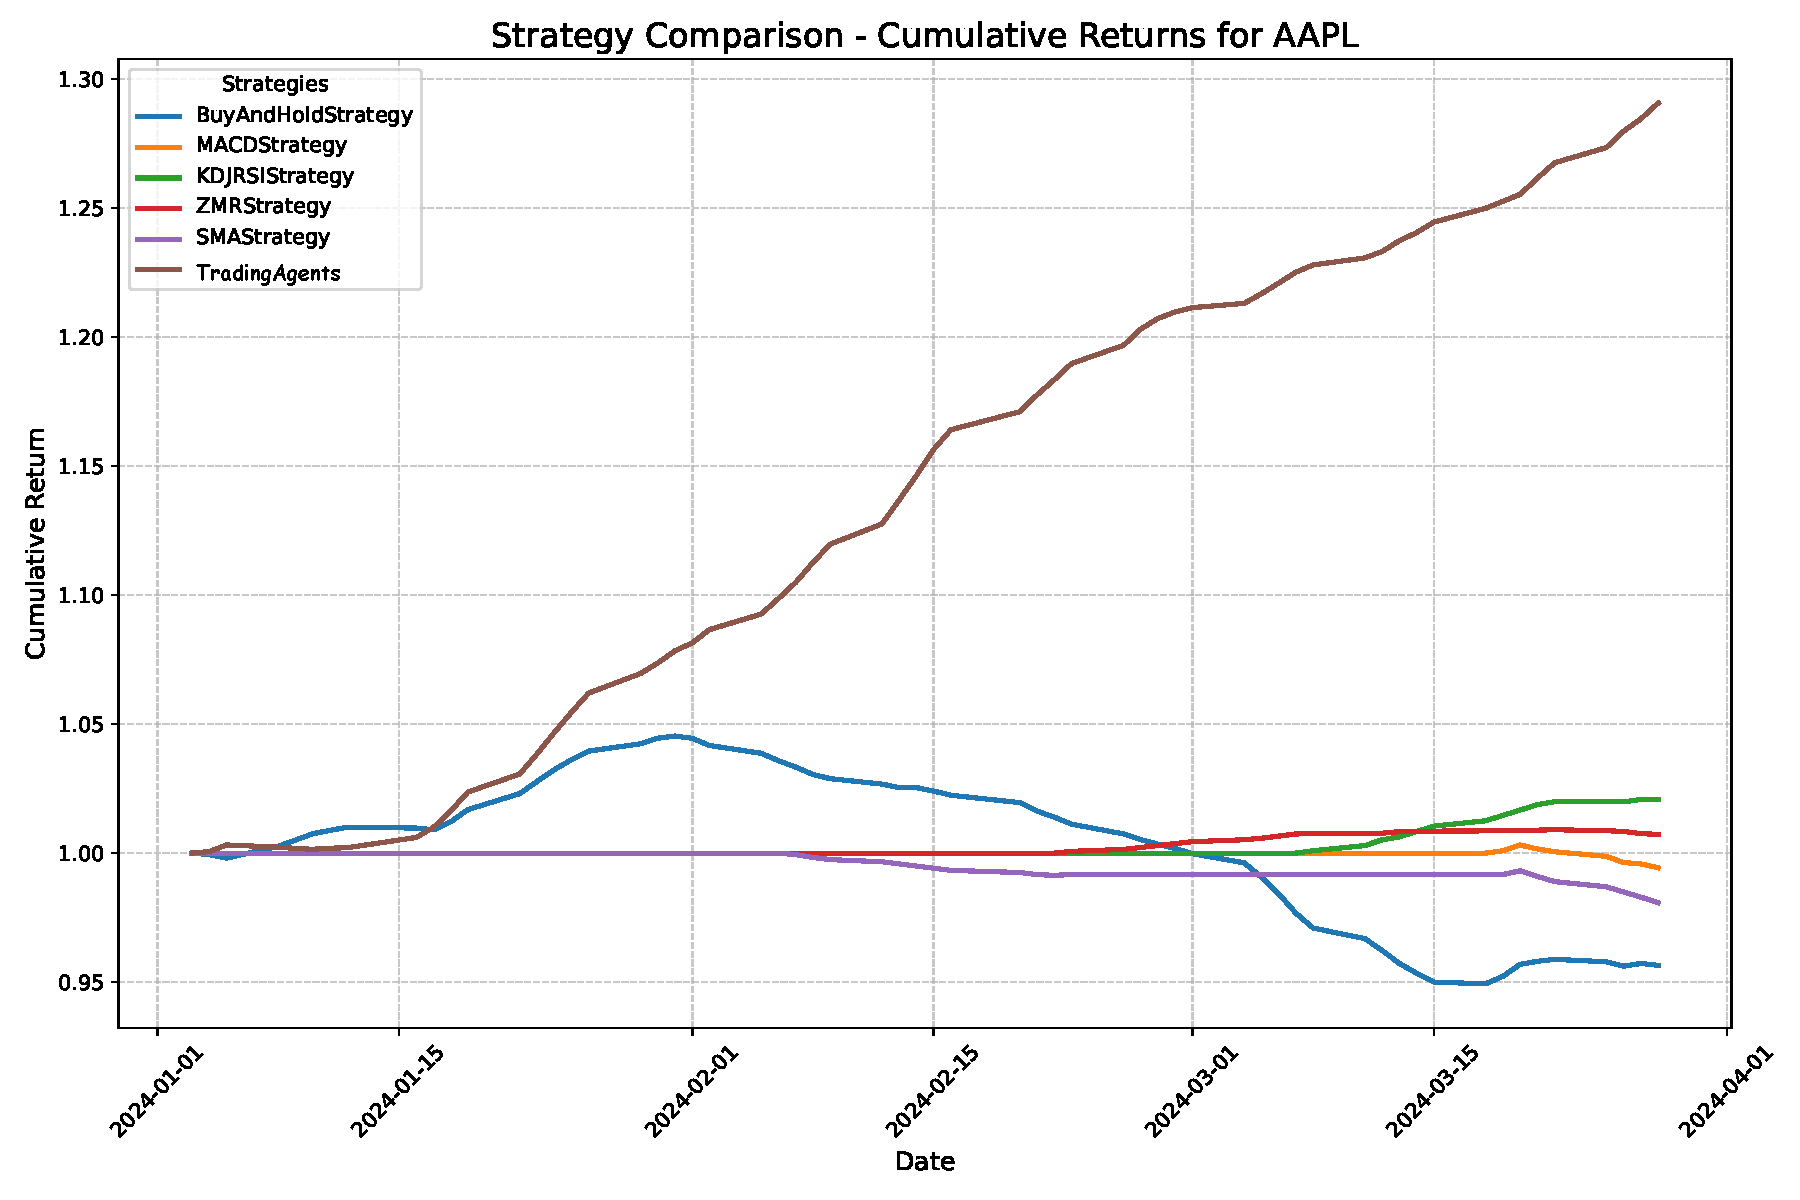
\includegraphics[width=0.75\columnwidth]{figures/AAPL/compare.pdf}}
\caption{Cumulative Returns on \$AAPL using \textbf{\textcolor{brown}{\model}}. The figure shows the performance comparison of our model against baseline approaches for Apple Inc. stock analysis.}
\label{fig:aapl-cumulative-returns}
\end{center}
\vskip -0.2in
\end{figure}

\vskip -1in

\subsubsection{Sharpe Ratio}

The Sharpe Ratio\footnote{We benchmarked \model over 3 months due to intensive LLM and tool use (11 LLM calls \& 20+ tool calls/prediction). The highest Sharpe Ratio exceeds our expected empirical range (\(SR\) above 2 -- very good, above 3 -- excellent). We exported \model's decision sequences and examined them to ensure calculation correctness. We believe the exceptionally high \(SR\) resulted from the phenomenon that there were few pullbacks in \model during that period. We report results as they are in our experiments faithfully. Future work will optimize LLM reasoning \& tool use to enable longer backtesting under limited budgets.}
 performance highlights \model's exceptional ability to deliver superior risk-adjusted returns, surpassing all baseline models. This result underscores \model's effectiveness in balancing returns and risk— a crucial factor for sustainable and predictable investment growth. \model outperforms market benchmarks such as Buy-and-Hold and rule-based strategies consistently, demonstrating its adaptability. Its capability to maximize returns while maintaining controlled risk exposure establishes a strong foundation for multi-agent and debate-based automated trading algorithms.

\subsubsection{Maximum Drawdown}
While rule-based baselines demonstrated superior performance in controlling risk, as reflected by their maximum drawdown scores, they fell short in capturing high returns. This trade-off between risk and reward underscores \model's strength as a balanced approach. Despite higher returns being typically associated with higher risks, \model maintained a relatively low maximum drawdown compared to many baselines. Its effective risk-control mechanisms, facilitated by the debates among risk-control agents, ensured that the maximum drawdown remained within a manageable limit, not exceeding 2. This demonstrates \model's capability to strike a robust balance between maximizing returns and managing risk effectively.

\subsubsection{Explainability}
A major drawback of current deep learning methods for trading is their dense, complex architectures, often rendering trading agents' decisions indecipherable. This challenge, rooted in AI explainability, is critical for trading agents operating in real-world financial markets, where incorrect decisions can cause severe losses. 

In contrast, an LLM-based agentic framework offers a transformative advantage: its decisions are communicated in natural language, enhancing interpretability. To illustrate, we provide \model's full trading log for a single day in the Appendix, showcasing its use of the ReAct-style prompting framework \citep{yao2023reactsynergizingreasoningacting}. Each decision includes detailed reasoning, tool usage, and thought processes, enabling traders to understand and debug the system. This transparency empowers traders to fine-tune the framework, accounting for decision factors, offering superior explainability over deep-learning trading algorithms.


\subsection{Discussion}
Our results demonstrate that integrating multiple specialized LLM agents and fostering agentic debate significantly enhances trading performance. This framework efficiently synthesizes diverse data sources and expert analyses, enabling trader agents to make well-informed decisions tailored to specific risk profiles. The inclusion of a reflective agent and a dedicated risk management team is pivotal in refining strategies and mitigating risks. As a result, the framework achieves exceptional return capture while maintaining strong risk management metrics, striking an optimal balance between maximizing rewards and minimizing risks. Additionally, the natural language-based operations of the multi-agent LLM framework ensure high explainability, giving \model a distinct advantage over traditional and deep learning methods in transparency and interoperability.


